\chapter{Experimentos numéricos}
\label{ch:chapter4}

Para medir el desempeño del algoritmo Newton-Lanczos se compara con otros dos métodos, el Análisis Discriminante Lineal (ADL) y la Regresión Logística Multinomial (RLM). Los criterios para elegir el mejor serán la tasa de reconocimiento y el tiempo de cómputo sobre los conjuntos de datos JAFFE y MNIST. Como el algoritmo de Newton-Lanczos ocupa los eigenvectores de una matriz, en la primer parte de este capítulo se medirá el tiempo de Lanczos y el costo de la rutina $SVD$ de R para una matriz en particular \footnote{La rutina $svd$ de $R$ ocupa la función $gesdd$ de la librería $LAPACK$. Para más información puede consultarse la página $http://www.netlib.org/lapack/$.}. En la segunda parte del capítulo, se explicará el preprocesamiento de las bases de datos y como se crearon los conjuntos de entrenamiento y prueba. En la tercer y cuarta parte, se realizan los experimentos con la bases de MNIST y JAFFE respectivamente. 

Para todos los experimentos de este capítulo, se utilizó el lenguaje de \textsf{R} en su versión 3.2.2 \textit{Fire Safety}. Los cálculos fueron realizados en una iMac 3.2 Ghz Intel Core i3 con 12 GB de RAM.

\section{Desempeño del método de Lanczos}

Antes de analizar el tiempo de cómputo de Newton-Lanczos, se evaluará el desempeño del algoritmo de Lanczos comparándolo con la factorización $svd$. Esto se realiza para saber en que casos es conveniente utilizar Lanczos y en cuales conviene calcular todos eigenpares. Para esta prueba se usó $A - \rho B$ con $A$ y $B$ las matrices de dispersión intra clase y entre clase de la base de datos MNIST y con $\rho = 3$. La siguiente gráfica resume el desempeño de ambos métodos.

\begin{figure}[!ht]
  \centering
  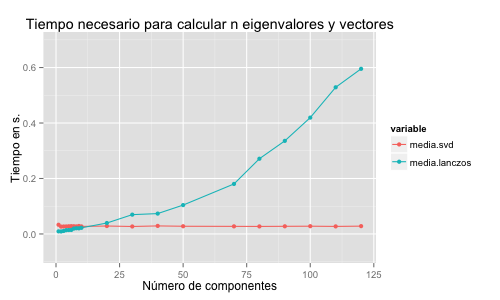
\includegraphics[width=1\textwidth]{Figures/Chapter4_eigen_lanczos.png} 
  \caption[Desempeño de Lanczos]
  {En el eje $x$ se representa k, el número de eigenpares a calcular de la matriz $A- \rho B$. La matriz original es de 193 x 193. El tiempo reportado para cada $k$, es el promedio de $30$ repeticiones para cada método.}
\end{figure}

En la figura 5.1 se observa que, para k menor a 10, el algoritmo de Lanczos es más rápido que la factorización $SVD$ de la matriz completa. Para valores más grandes, conviene factorizar toda la matriz. Esto puede deberse a que en aritmética inexacta Lanczos presenta el problema de \textit{Ghost eigenvalues} (eigenvalores que se repiten, pero que son espurios) \cite{golub2012matrix}. Estos se originan porque la ortogonalidad entre los eigenvectores se pierde conforme la dimensionalidad aumenta. Para solucionar este problema, se realizó una reortogonalización completa en cada iteración, lo que pudo aumentar el tiempo de cómputo. 

\section{Modelos comparados y preprocesamiento de las bases}

En este capítulo el método de Newton-Lanczos se comparó con la RLM y con el ADL. Para el primero, se usó la función \textit{multinom} del paquete \textit{nnet}, mientras que para el segundo se utilizó una modificación de la función \textit{lda} \footnote{La modificación está presentada en los códigos del apéndice B} del paquete \textit{MASS}. Ambas funciones fueron desarrolladas por Brian Ripley, profesor de estadística aplicada de la Universidad de Oxford. 

Como primer paso se definieron los tamaños del conjunto de entrenamiento y prueba. Para el entrenamiento de MNIST se ocuparon 4000 datos (400 por clase); es decir, el 6\% del total. En el caso de JAFFE se utilizaron 50 datos (5 por clase); es decir, el 23\% del total. En ambos, el resto de los datos se ocupó en el conjunto de prueba. 

Para el preprocesamiento de las bases, cada imagen se convirtió en un vector con tamaño asociado al número de pixeles. Esto genera un problema con dimensiones altas, por lo que se realizó un paso de reducción dimensional. Se tomaron las primeras componentes principales (PCA) del conjunto de entrenamiento de manera que se explicara el 95\% de la varianza total, después se proyectó el conjunto de prueba. Para el ejemplo de MNIST se tomaron 193 de las 784 componentes; en cambio, para JAFFE se tomaron 50 de las 65536. 

Una vez hecho el preprocesamiento, se realizaron 2 experimentos para cada base de datos. Para el primero se utilizó el método de Newton-Lanczos y se proyectaron los datos de entrenamiento a una dimensión (k) igual a 20. Los objetivos de este fueron los siguientes: 

\begin{itemize}
\item Ejemplificar las cotas para $\rho^*$
\item Analizar como cambia el valor de $f(\rho)$ con el método de Newton-Lanczos
\item Ver como se ven proyectados los datos en dimensiones menores
\end{itemize}

En el segundo experimento se entrenaron los 3 métodos con distintas $k$. Después se midió la tasa de reconocimiento alcanzada (usando el conjunto de prueba) y su tiempo de ejecución. 

\section{Base de datos MNIST}

Las siglas MNIST provienen de (\textit{Mixed National Institute of Standards and Technology}), la cual contiene datos de 70,000 dígitos escritos a mano que se usan comúnmente para probar códigos de clasificación de imágenes. De esta manera, en el experimento se tendrán 10 clases: los dígitos del 0-10. La base de datos surge de la colaboración de Yann LeCun del Instituto Courant (NYU), de Corinna Cortes de Google Labs (NY) y de Christopher J.C. Burges de Microsoft Research en Redmond. Puede descargarse de la página Web \textit{yann.lecun.com/exdb/mnist}, cuyo link sigue vigente al 13 de marzo del 2016.

Las imágenes están en un formato especial llamado IDX. Para poderlas convertir en un archivo leíble para R, se utilizó la función \textit{readMNIST} del paquete \textit{darch}. Esta paquetería convierte los archivos a objetos \textit{.RData}. La siguiente figura contiene una extracto de tamaño 225 de todo el conjunto.

\begin{figure}[!ht]
  \centering
	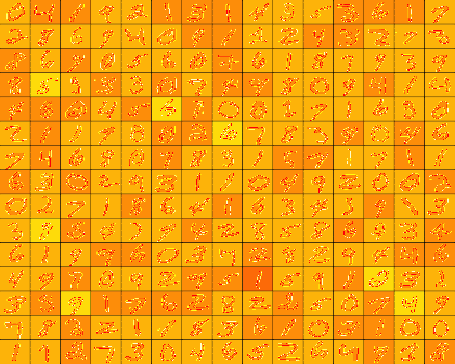
\includegraphics[width=1\textwidth]{Figures/Chapter4_numeros.png}	
  \caption{Ejemplo de números de la base de datos (MNIST).}
\end{figure}

\subsection{Proyección sobre un espacio de dimensión 20}

\underline{\textbf{1) Cotas para $\rho^*$}}

En el capítulo 2 se presentaron cotas para $\rho^*$ y en esta sección se ejemplificará la segunda de ellas para esta base de datos. Se calcularon los eigenvalores de la matriz intraclase (B) y de la matriz entre clases (A). Los 20 eigenvalores más grandes y más pequeños de la primera son \footnote{los eigenvalores menores a $1e^{-10}$ se consideraron numéricamente como 0}:

\begin{center}
\begin{tabular}{ | c | c|  c |c | c|  c |c | c|  c |c | c | c|  c |c | c|  c |c | c|  c |c |} 
\hline
12694 & 10367 & 7822 & 6793 & 6013 & 5887 & 5269 & 4704 & 4474 & 3969 \\
3833 & 3428 & 3124 & 3015 & 2978 & 2627 & 2535 & 2353 & 2232 & 2150 \\
\hline
\hline
\end{tabular}
\end{center}

\begin{center}
\begin{tabular}{ | c | c|  c |c | c|  c |c | c|  c |c | c | c|  c |c | c|  c |c | c|  c |c |} 
\hline
73 & 72 & 72 & 71 & 71 & 70 & 70 & 69 & 68 & 68 \\
67 & 67 & 66 & 66 & 65 & 64 & 64 & 63 & 63 & 62 \\
\hline
\hline
\end{tabular}
\end{center}

Mientras que los 9 eigenvalores más grandes de la matriz entre clases (A) son (los demás son 0):

\begin{center}
\begin{tabular}{ | c | c|  c |c | c|  c |c | c|  c |} 
\hline
12865 & 9821 & 7408 & 4736 & 3558 & 2312 & 1879 & 885 & 631 \\
\hline
\hline
\end{tabular}
\end{center}

Sustituyendo estos valores en la fórmula de las cotas de la raíz, se tiene que:

\begin{equation*}
\frac{\sum_{i = 1}^{p}\lambda_{A_i}}{\sum_{i = 1}^{p}\lambda_{B_i}} \leq \rho^* \leq \frac{\sum_{i = 1}^{p}\lambda_{(A)_i}}{\sum_{i = 1}^{p}\lambda_{(B)_{n-i+1}}}	
\end{equation*}

\begin{equation*}
\frac{44099.28}{96277.31} \leq \rho^* \leq \frac{44099.28}{1364.54}
\end{equation*}

\begin{equation*}
0.4580443 \leq \rho^* \leq 32.31806
\end{equation*}

\underline{\textbf{2) Valores de $(\rho^*, f(\rho))$}}

Para el punto inicial de este experimento se utilizará el punto medio del intervalo. Los criterios de paro se fijaron con una tolerancia de $1e^{-10}$ y que las iteraciones sean menor a 50. Con este ejemplo, se obtienen los siguientes resultados para $\rho$ y $f(\rho)$:

\begin{center}
\begin{tabular}{ | c | c|  c |} 
\hline
$iter$ & $\rho$ & $f(\rho)$  \\ 
\hline
\hline
1 & $16.38805180$ & $-22,326.51$  \\ 
\hline
2 & $0.03121373$ & $42,841.16$  \\ 
\hline
3 & $1.11003833$ & $15,197.50$  \\ 
\hline
4 & $2.05957127$ & $3,926.463$  \\ 
\hline
5 & $2.50843464$ & $444.8128$  \\ 
\hline
6 & $2.57388828$ & $9.007894$  \\ 
\hline
7 & $2.57526971$ & $.004008613$  \\ 
\hline
8 & $2.57527033$ & $7.891856e^{-10}$  \\ 
\hline
9 & $2.57527033$ & $5.371703e^{-12}$  \\ 
\hline
\hline

\end{tabular}
\end{center}

En la figura 5.3 se muestran $(\rho, f(\rho))$. El punto inicial es el rojo, en este caso $\rho = 16.3880$, mientras que $f(\rho)$ toma el valor de $-22,326.51$. Tras la primer iteración, $\rho$ toma el valor de $0.0312$, y $f(\rho)$ es igual $42,841.16$. Conforme hay más iteraciones, el cambio de $\rho$ disminuye, hasta converger a un óptimo. En el ejemplo resulta ser $2.57527033$. Con esta $\rho$, $f(\rho)$ debe tomar el valor de 0, pero toma el valor de $5.371703e^{-12}$, ya que nuestro nivel de tolerancia para detener el algoritmo es $1e^{-10}$.

\begin{figure}[!ht]
  \centering
	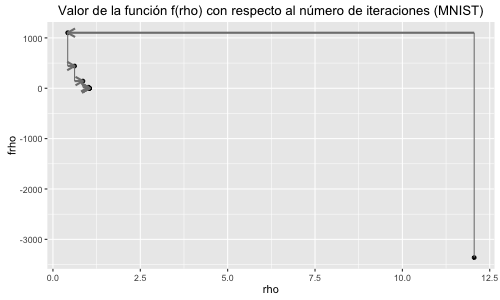
\includegraphics[width=1\textwidth]{Figures/Chapter4_Iteraciones.png}	
  \caption{Valores de $\rho$ y $f(\rho)$ para distintas iteraciones (MNIST).}
\end{figure}

\pagebreak
\underline{\textbf{3) Datos proyectados en 4 dimensiones}}

Se maximizó la traza del cociente para un espacio de 20 dimensiones. En la figura 5.4 se muestra como se agrupan los individuos del conjunto de entrenamiento conforme las iteraciones avanzan. 
  
\begin{figure}[!ht]
  \centering
	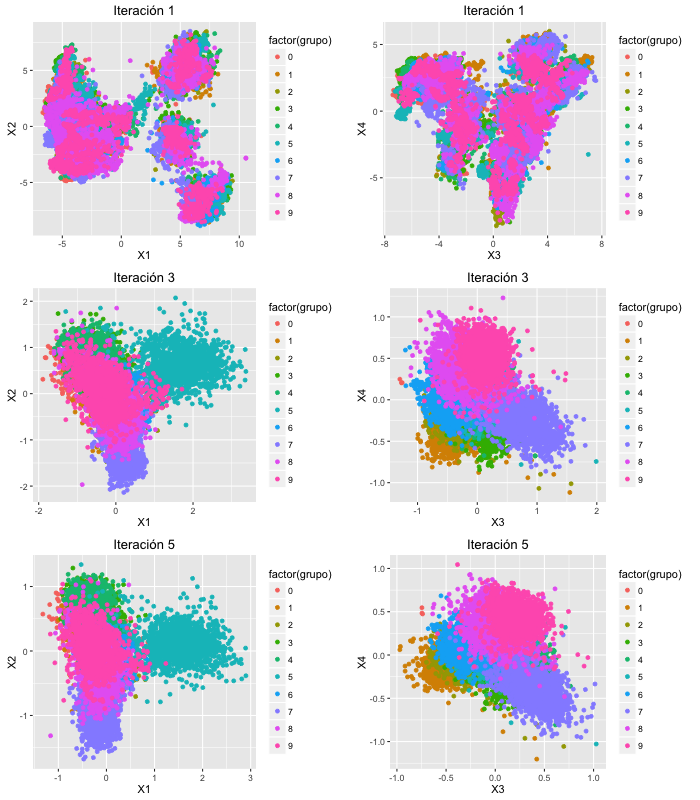
\includegraphics[width=1\textwidth]{Figures/Chapter4_ejemplo20componentes.png}	
  \caption[Ejemplo de proyección en 20 dimensiones (MNIST)]
  {Las dos imágenes superiores son los datos de entrenamiento proyectadas sobre las 4 primeras componentes tras la primer iteración. Las dos intermedias son en la iteración 3 y las últimas 2 son la última iteración.}
\end{figure}

\pagebreak

\subsection{Comparación con otros métodos}

Para la comparación de Newton-Lanczos con la RLM y el ADL se tomaron las siguientes consideraciones:

\begin{itemize}
\item Las dimensiones a considerar (k) son: 2, 5, 10, 15, 20, 40, 60, 80, 100, 120, 140, 160, 180 y 193
\item El número de variables que entran en cada modelo es el mismo (dada la dimensión k)
\item Los modelos se ajustan con el conjunto de entrenamiento y se calcula el error con el de prueba
\item Para Newton-Lanczos y ADL se proyectarán a un espacio k-dimensional y se usará 3-vecinos más cercanos para clasificarlos
\item Para el caso de regresión logística multinomial se eligirá la clase que tenga una mayor probabilidad posterior de selección
\end{itemize}

\underline{\textbf{1) Tasa de reconocimiento}}

La tasa de reconocimiento se mide como el número de individuos clasificados correctamente entre el número total del conjunto de test. Como el objetivo de esta sección es observar como se modifica la tasa con respecto aumenta k, se fijo el número de vecinos más cercanos a 3 para el caso de ADL y de Newton-Lanczos y también el tamaño del conjunto de entrenamiento. En la figura 5.5 se muestra que el modelo RLM y el ADL se comportan mejor para dimensiones pequeñas. Para casos de k mayor a 120, el método de Newton-Lanczos alcanza una mejor tasa de reconocimiento.

Es interesante observar que si se busca la mejor proyección con para k = 1 y k = 2, Newton-Lanczos resulta ser muy buen método. En la figura 5.4 se observó como los individuos se agrupan con este método. 
\pagebreak

\begin{figure}[!ht]
  \centering
	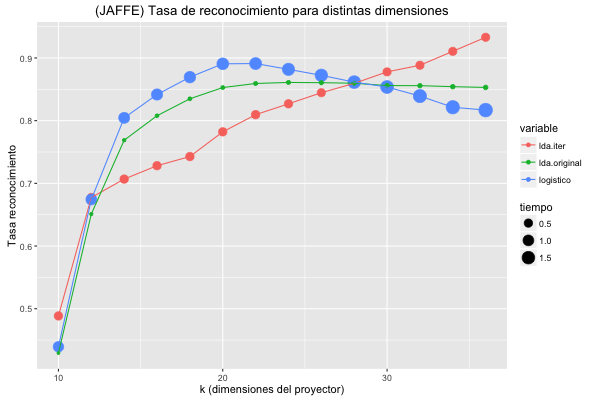
\includegraphics[width=1\textwidth]{Figures/Chapter4_Comparacion.png}	
  \caption[Tasa de reconocimiento base (MNIST)]
  {En azul se representa el RLM, en verde el ADL y en rojo el método de Newton-Lanczos. En el eje $y$ se muestra la tasa de reconocimiento y en el eje $x$ la dimensión a considerar (k). El tamaño representa el tiempo.}
\end{figure}

\underline{\textbf{2) Tiempo de ejecución}}

A continuación, se comparan los tiempos de ejecución de cada método. Para comparar los tiempos de ejecución justamente, se tomaron 3 distintos:

\begin{itemize}
\item 1) (PCA) Tiempo para calcular los componentes principales del conjunto de entrenamiento
\item 2) (Proyectar) Tiempo para calcular la proyección del conjunto de test
\item 3) (Modelo) Tiempo necesario para hacer las operaciones de cada método

\end{itemize}

\begin{center}
\begin{tabular}{ | c | c |} 
\hline
 PCA(s) & Proyectar(s) \\ 
\hline
\hline
$11.728$ & $21.680$ \\ 
\hline
\hline
\end{tabular}
\end{center}


\begin{center}
\begin{tabular}{ | c | c | c | c | c | c | c | c |} 
\hline
Comp & lda.iter & logístico & lda.orig   & Comp & lda.iter & logístico & lda.orig   \\ 
\hline
\hline
$2$ & $0.9092$ & $0.2712$ & $0.01$ & $80$ & $0.9222$ & $4.3186$ & $0.2684$ \\
$5$ & $0.8576$ & $0.5188$ & $0.0466$ & $100$ & $0.8764$ & $5.6474$ & $0.3572$ \\
$10$ & $0.864$ & $1.0646$ & $0.025$ & $120$ & $0.8952$ & $8.1026$ & $0.4942$ \\
$15$ & $0.8768$ & $1.103$ & $0.0372$ & $140$ & $0.9016$ & $9.2944$ & $0.7902$ \\
$20$ & $0.8886$ & $1.2888$ & $0.0524$ & $160$ & $0.8782$ & $10.1534$ & $0.908$ \\
$40$ & $0.886$ & $2.5528$ & $0.1004$ & $180$ & $0.898$ & $12.0426$ & $1.0596$ \\
$60$ & $0.8728$ & $3.2034$ & $0.1744$ & $193$ & $0643$ & $14.2512$ & $1.2186$ \\
\hline
\hline
\end{tabular}
\end{center}

El tiempo está en segundos (s).

Para cada iteración del método de Newton-Lanczos, se calcularon todos los eigenvalores ya que al no calcularlos, solo se tendrá una aproximación a sus valores y sus eigenvectores. Por este motivo, se decidió sacrificar tiempo de cómputo por precisión.

\section{Base de datos JAFFE}


Ahora se analizará la base JAFFE \textit{Japanese Female Facial Expression}, que consta de 213 fotos provenientes de 10 personas distintas. Este conjunto de datos fue creado inicialmente para clasificar emociones, pero se usa comúnmente para probar otros tipos de algoritmos de clasificación. En nuestro caso será usado para clasificar el rostro de la persona, de esta manera se tendrán 10 clases. La base fue creada por Michael Lyons, Miyuki Kamachi y Jiro Gyoba en el departamento de psicología de la universidad de Kyushu. Puede descargarse de la página Web \textit{www.kasrl.org/jaffe.html}, cuyo link sigue vigente al 13 de marzo del 2016.

Las imágenes se encuentran en un formato \textit{.tiff}, por lo que se requirió la función \textit{readTIFF} del paquete $tiff$ el cual permite leerlas y convertirlas en un formato \textit{.RData}. La figura 5.6 contiene un extracto de tamaño 35 de la base original.

\pagebreak

\begin{figure}[!ht]
  \centering
  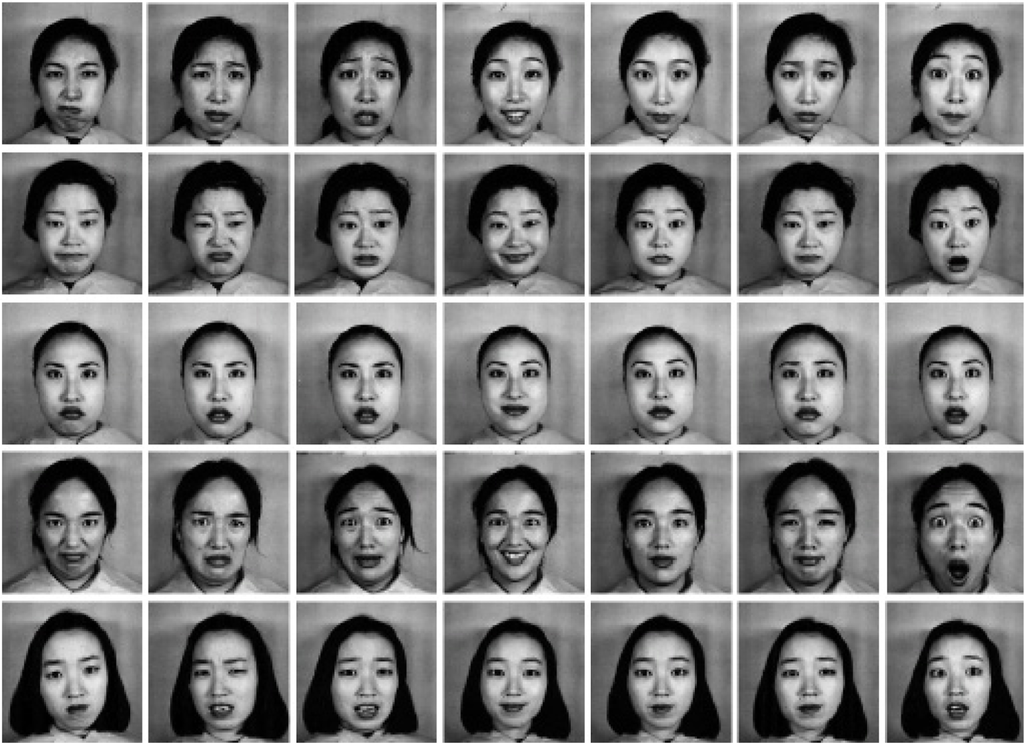
\includegraphics[width=.8\textwidth]{Figures/Chapter4_Jaffe.png} 
  \caption{Ejemplo de la base de datos (JAFFE).}
\end{figure}

\subsection{Proyección sobre un espacio de dimensión 20}

\underline{\textbf{1) Cotas para $\rho^*$}}

Al igual que el ejemplo de MNIST, se ejemplificará la segunda cota presentada en el capítulo 2. Para esto se calcularon los eigenvalores de la matriz intraclase (B) y de la matriz entre clases (A). Los 20 eigenvalores más grandes y más pequeños de la primera son: \footnote{los eigenvalores menores a $1e^{-10}$ se consideraron numéricamente como 0}

\begin{center}
\begin{tabular}{ | c | c|  c |c | c|  c |c | c|  c |c | c | c|  c |c | c|  c |c | c|  c |c |} 
\hline
5303 & 4627 & 2083 & 1556 & 1370 & 1177 & 851 & 781 & 740 & 705 \\
629 & 596 & 562 & 520 & 498 & 466 & 453 & 403 & 397 & 382 \\
\hline
\hline
\end{tabular}
\end{center}

\begin{center}
\begin{tabular}{ | c | c|  c |c | c|  c |c | c|  c |c | c | c|  c |c | c|  c |c | c|  c |c |} 
\hline
250 & 245 & 231 & 223 & 219 & 203 & 198 & 192 & 176 & 147 \\
141 & 0 & 0 & 0 & 0 & 0 & 0 & 0 & 0 & 0 \\
\hline
\hline
\end{tabular}
\end{center}

De la misma manera, se calculan los 9 eigenvalores más grandes de la matriz entre clases (Los demás son 0):

\begin{center}
\begin{tabular}{ | c | c|  c |c | c|  c |c | c|  c |} 
\hline
14051 & 12922 & 7775 & 3247 & 3138 & 2849 & 1918 & 1336 & 1317 \\
\hline
\hline
\end{tabular}
\end{center}

Usando las formulas del capítulo 2, se tienen las siguientes cotas para $\rho^*$:

\begin{equation*}
\frac{\sum_{i = 1}^{p}\lambda_{A_i}}{\sum_{i = 1}^{p}\lambda_{B_i}} \leq \rho^* \leq \frac{\sum_{i = 1}^{p}\lambda_{(A)_i}}{\sum_{i = 1}^{p}\lambda_{(B)_{n-i+1}}}  
\end{equation*}

\begin{equation*}
\frac{48553}{24099} \leq \rho^* \leq \frac{48553}{2225}
\end{equation*}

\begin{equation*}
2.0147 \leq \rho^* \leq 21.8216
\end{equation*}



\underline{\textbf{2) Valores de $(\rho^*, f(\rho^*))$}}

Los criterios de paro se fijaron iguales que el ejemplo pasado (tol: $1e^{-10}$ y menos de 50 iteraciones). Para la base de JAFFE, se encontraron los siguientes resultados:

\begin{center}
\begin{tabular}{ | c | c|  c |} 
\hline
$iter$ & $\rho$ & $f(\rho)$  \\ 
\hline
\hline
1 & $11.88493$ & $6093.742$  \\ 
\hline
2 & $14.33840$ & $80.44169$  \\ 
\hline
3 & $14.37160$ & $.01093739e$  \\ 
\hline
4 & $14.37161$ & $1.873559 e^{-10}$  \\ 
\hline
\hline
\end{tabular}
\end{center}

\begin{figure}[!ht]
  \centering
  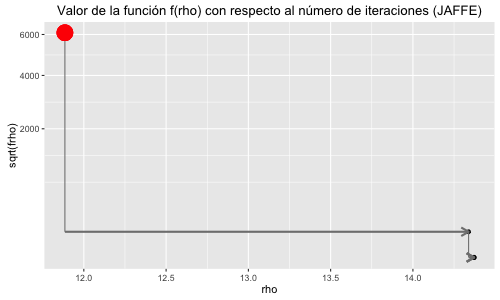
\includegraphics[width=.75 \textwidth]{Figures/Chapter4_Iteraciones_JAF.png} 
  \caption{Valores de $\rho$ y $f(\rho)$ para las iteraciones (JAFFE).}
\end{figure}

Se ve que la convergencia cuadrática del método de Newton ayuda a que se alcance el óptimo en pocas iteraciones. En la cuarta iteración $f(\rho)$ ya toma el valor de $1.87 e^{-10}$, muy cercano a 0. 

\underline{\textbf{3) Datos proyectados en 4 dimensiones}}

De nuevo se maximizó la traza del cociente para un espacio de 20 dimensiones. En la figura 5.8 se muestra como se agrupan los individuos del conjunto de entrenamiento conforme las iteraciones avanzan.

\begin{figure}[!ht]
  \centering
  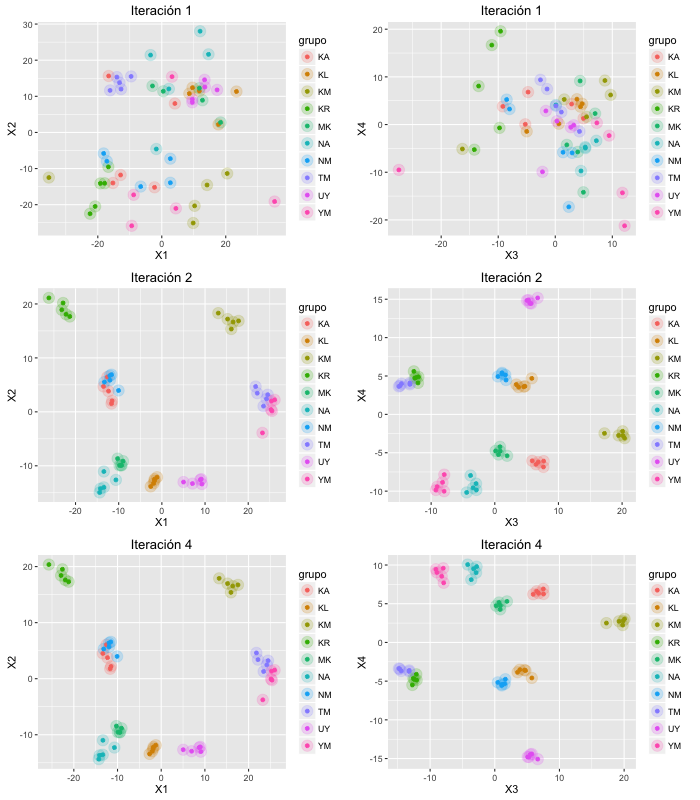
\includegraphics[width=1\textwidth]{Figures/Chapter4_ejemplo20componentes_JAF.png} 
  \caption[Ejemplo de proyección en 20 dimensiones (MNIST)]
  {Las dos imágenes superiores son los datos de entrenamiento proyectadas sobre las 4 primeras componentes tras la primer iteración. Las dos intermedias son en la iteración 3 y las últimas 2 son la última iteración.}
\end{figure}


\subsection{Comparación con otros métodos}

De la misma forma que el ejemplo pasado se compararon los métodos en este caso. Lo único distinto serán las dimensiones a considerar k = 10, 13, 16, 19, 22, 25, 28, 31, 34, 37, 40, 43, 46 y 49. 

\underline{\textbf{1) Tasa de reconocimiento}}

\begin{figure}[!ht]
  \centering
  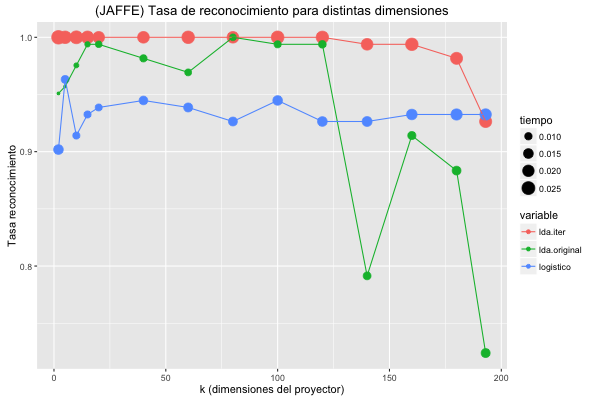
\includegraphics[width=1\textwidth]{Figures/Chapter4_Comparacion_Jaf.png} 
  \caption[Comportamiento de los 3 métodos comparados (JAFFE)]
  {En azul se representa el RLM, en verde el ADL y en rojo el método de Newton-Lanczos. En el eje $y$ se muestra la tasa de reconocimiento y en el eje $x$ la dimensión a considerar (k). El tamaño representa el tiempo. Se observa que en el ADL los últimos 4 puntos bajan la predicción. Esto es porque las variables son colineales y al calcular la inversa, causa inestabilidad numérica.}
\end{figure}

En la figura 5.9 se observa que el método de lda iterativo no tiene ningún error de clasificación para espacios de proyección menor a 40 dimensiones, reduciéndose en espacios de proyección con dimensión más alta. Esto puede deberse a que las últimas componentes son las menos discriminadoras, pero el método de 3-vecinos más cercanos las pondera igual. Una posible modificación que se puede realizar, es ponderar cada componente de acuerdo al poder discriminativo del correspondiente eigenvector.

En la figura 5.10 se muestran las últimas 4 componentes. Se observa que los individuos ya no están tan agrupados como en las primeras 4, por lo que el clasificador de 3-vecinos más cercanos podría no estar funcionando bien para $k > 40$.

\begin{figure}[!ht]
  \centering
  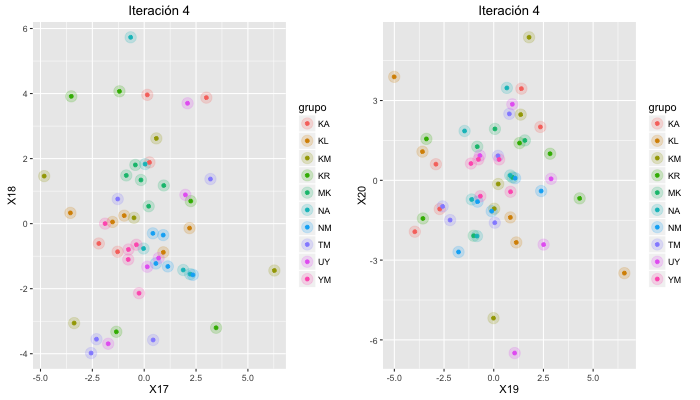
\includegraphics[width=.95\textwidth]{Figures/Chapter4_ultimasComponentes_JAF.png} 
  \caption[Individuos proyectados (JAFFE)]
  {Conjunto de entrenamiento proyectados sobre las ultimas 4 componentes (17,18,19,20). Se observa que los grupos siguen estando relativamente cerca, pero si se toma 3-vecinos más cercanos no necesariamente se escogerá la persona correcta.}
\end{figure}


\underline{\textbf{2) Tiempo de ejecución}}
A continuación, se comparan los tiempos de ejecución de cada método. Para compararlos justamente, se tomaron 3 fases distintas y se comparó solamente el tiempo del modelo.

\begin{itemize}
\item 1) (PCA) Tiempo para calcular los componentes principales del conjunto de entrenamiento
\item 2) (Proyectar) Tiempo para calcular la proyección del conjunto de test
\item 3) (Modelo) Tiempo necesario para hacer las operaciones de cada método

\end{itemize}

\begin{center}
\begin{tabular}{ | c | c |} 
\hline
 PCA(s) & Proyectar(s) \\ 
\hline
\hline
$4.666$ & $4.801$ \\ 
\hline
\hline
\end{tabular}
\end{center}


\begin{center}
\begin{tabular}{ | c | c | c | c | c | c | c | c |} 
\hline
Comp & lda.iter & logístico & lda.orig   & Comp & lda.iter & logístico & lda.orig   \\ 
\hline
\hline
$10$ & $0.0352$ & $0.0098$ & $0.0068$ & $31$ & $0.0312$ & $0.0436$ & $0.0136$ \\
$13$ & $0.0324$ & $0.0146$ & $0.0074$ & $34$ & $0.0314$ & $0.0176$ & $0.0134$ \\
$16$ & $0.0378$ & $0.018$ & $0.0082$ & $37$ & $0.0314$ & $0.0224$ & $0.0144$ \\
$19$ & $0.031$ & $0.0114$ & $0.0104$ & $40$  & $0.0312$ & $0.0266$ & $0.0152$ \\
$22$ & $0.0308$ & $0.0128$ & $0.0112$ & $43$ & $0.0294$ & $0.0248$ & $0.0164$ \\
$25$ & $0.0326$ & $0.0136$ & $0.0102$ & $46$ & $0.03$ & $0.0228$ & $0.0188$ \\
$28$ & $0.0318$ & $0.0158$ & $0.0112$ & $49$ & $0.0204$ & $0.0594$ & $0.0176$ \\
\hline
\hline
\end{tabular}
\end{center}

El tiempo está en segundos (s).

Para cada iteración del método de Newton-Lanczos, se calcularon todos los eigenvalores ya que al no calcular todos, solo se tendrá una aproximación a sus valores y sus eigenvectores. Por este motivo, se decidió sacrificar tiempo de cómputo por precisión.



